% Options for packages loaded elsewhere
\PassOptionsToPackage{unicode}{hyperref}
\PassOptionsToPackage{hyphens}{url}
%
\documentclass[
]{book}
\title{Creating Migratory Networks in R}
\author{Matt DeSaix}
\date{2022-01-05}

\usepackage{amsmath,amssymb}
\usepackage{lmodern}
\usepackage{iftex}
\ifPDFTeX
  \usepackage[T1]{fontenc}
  \usepackage[utf8]{inputenc}
  \usepackage{textcomp} % provide euro and other symbols
\else % if luatex or xetex
  \usepackage{unicode-math}
  \defaultfontfeatures{Scale=MatchLowercase}
  \defaultfontfeatures[\rmfamily]{Ligatures=TeX,Scale=1}
\fi
% Use upquote if available, for straight quotes in verbatim environments
\IfFileExists{upquote.sty}{\usepackage{upquote}}{}
\IfFileExists{microtype.sty}{% use microtype if available
  \usepackage[]{microtype}
  \UseMicrotypeSet[protrusion]{basicmath} % disable protrusion for tt fonts
}{}
\makeatletter
\@ifundefined{KOMAClassName}{% if non-KOMA class
  \IfFileExists{parskip.sty}{%
    \usepackage{parskip}
  }{% else
    \setlength{\parindent}{0pt}
    \setlength{\parskip}{6pt plus 2pt minus 1pt}}
}{% if KOMA class
  \KOMAoptions{parskip=half}}
\makeatother
\usepackage{xcolor}
\IfFileExists{xurl.sty}{\usepackage{xurl}}{} % add URL line breaks if available
\IfFileExists{bookmark.sty}{\usepackage{bookmark}}{\usepackage{hyperref}}
\hypersetup{
  pdftitle={Creating Migratory Networks in R},
  pdfauthor={Matt DeSaix},
  hidelinks,
  pdfcreator={LaTeX via pandoc}}
\urlstyle{same} % disable monospaced font for URLs
\usepackage{color}
\usepackage{fancyvrb}
\newcommand{\VerbBar}{|}
\newcommand{\VERB}{\Verb[commandchars=\\\{\}]}
\DefineVerbatimEnvironment{Highlighting}{Verbatim}{commandchars=\\\{\}}
% Add ',fontsize=\small' for more characters per line
\usepackage{framed}
\definecolor{shadecolor}{RGB}{248,248,248}
\newenvironment{Shaded}{\begin{snugshade}}{\end{snugshade}}
\newcommand{\AlertTok}[1]{\textcolor[rgb]{0.94,0.16,0.16}{#1}}
\newcommand{\AnnotationTok}[1]{\textcolor[rgb]{0.56,0.35,0.01}{\textbf{\textit{#1}}}}
\newcommand{\AttributeTok}[1]{\textcolor[rgb]{0.77,0.63,0.00}{#1}}
\newcommand{\BaseNTok}[1]{\textcolor[rgb]{0.00,0.00,0.81}{#1}}
\newcommand{\BuiltInTok}[1]{#1}
\newcommand{\CharTok}[1]{\textcolor[rgb]{0.31,0.60,0.02}{#1}}
\newcommand{\CommentTok}[1]{\textcolor[rgb]{0.56,0.35,0.01}{\textit{#1}}}
\newcommand{\CommentVarTok}[1]{\textcolor[rgb]{0.56,0.35,0.01}{\textbf{\textit{#1}}}}
\newcommand{\ConstantTok}[1]{\textcolor[rgb]{0.00,0.00,0.00}{#1}}
\newcommand{\ControlFlowTok}[1]{\textcolor[rgb]{0.13,0.29,0.53}{\textbf{#1}}}
\newcommand{\DataTypeTok}[1]{\textcolor[rgb]{0.13,0.29,0.53}{#1}}
\newcommand{\DecValTok}[1]{\textcolor[rgb]{0.00,0.00,0.81}{#1}}
\newcommand{\DocumentationTok}[1]{\textcolor[rgb]{0.56,0.35,0.01}{\textbf{\textit{#1}}}}
\newcommand{\ErrorTok}[1]{\textcolor[rgb]{0.64,0.00,0.00}{\textbf{#1}}}
\newcommand{\ExtensionTok}[1]{#1}
\newcommand{\FloatTok}[1]{\textcolor[rgb]{0.00,0.00,0.81}{#1}}
\newcommand{\FunctionTok}[1]{\textcolor[rgb]{0.00,0.00,0.00}{#1}}
\newcommand{\ImportTok}[1]{#1}
\newcommand{\InformationTok}[1]{\textcolor[rgb]{0.56,0.35,0.01}{\textbf{\textit{#1}}}}
\newcommand{\KeywordTok}[1]{\textcolor[rgb]{0.13,0.29,0.53}{\textbf{#1}}}
\newcommand{\NormalTok}[1]{#1}
\newcommand{\OperatorTok}[1]{\textcolor[rgb]{0.81,0.36,0.00}{\textbf{#1}}}
\newcommand{\OtherTok}[1]{\textcolor[rgb]{0.56,0.35,0.01}{#1}}
\newcommand{\PreprocessorTok}[1]{\textcolor[rgb]{0.56,0.35,0.01}{\textit{#1}}}
\newcommand{\RegionMarkerTok}[1]{#1}
\newcommand{\SpecialCharTok}[1]{\textcolor[rgb]{0.00,0.00,0.00}{#1}}
\newcommand{\SpecialStringTok}[1]{\textcolor[rgb]{0.31,0.60,0.02}{#1}}
\newcommand{\StringTok}[1]{\textcolor[rgb]{0.31,0.60,0.02}{#1}}
\newcommand{\VariableTok}[1]{\textcolor[rgb]{0.00,0.00,0.00}{#1}}
\newcommand{\VerbatimStringTok}[1]{\textcolor[rgb]{0.31,0.60,0.02}{#1}}
\newcommand{\WarningTok}[1]{\textcolor[rgb]{0.56,0.35,0.01}{\textbf{\textit{#1}}}}
\usepackage{longtable,booktabs,array}
\usepackage{calc} % for calculating minipage widths
% Correct order of tables after \paragraph or \subparagraph
\usepackage{etoolbox}
\makeatletter
\patchcmd\longtable{\par}{\if@noskipsec\mbox{}\fi\par}{}{}
\makeatother
% Allow footnotes in longtable head/foot
\IfFileExists{footnotehyper.sty}{\usepackage{footnotehyper}}{\usepackage{footnote}}
\makesavenoteenv{longtable}
\usepackage{graphicx}
\makeatletter
\def\maxwidth{\ifdim\Gin@nat@width>\linewidth\linewidth\else\Gin@nat@width\fi}
\def\maxheight{\ifdim\Gin@nat@height>\textheight\textheight\else\Gin@nat@height\fi}
\makeatother
% Scale images if necessary, so that they will not overflow the page
% margins by default, and it is still possible to overwrite the defaults
% using explicit options in \includegraphics[width, height, ...]{}
\setkeys{Gin}{width=\maxwidth,height=\maxheight,keepaspectratio}
% Set default figure placement to htbp
\makeatletter
\def\fps@figure{htbp}
\makeatother
\setlength{\emergencystretch}{3em} % prevent overfull lines
\providecommand{\tightlist}{%
  \setlength{\itemsep}{0pt}\setlength{\parskip}{0pt}}
\setcounter{secnumdepth}{5}
\usepackage{booktabs}
\ifLuaTeX
  \usepackage{selnolig}  % disable illegal ligatures
\fi
\usepackage[]{natbib}
\bibliographystyle{plainnat}

\begin{document}
\maketitle

{
\setcounter{tocdepth}{1}
\tableofcontents
}
\hypertarget{introduction}{%
\chapter{Introduction}\label{introduction}}

This text outlines how to create migratory networks using the R package \texttt{MuSpTest} (\emph{We need a name!}). The creation of the migratory networks is broken into three main parts:

\begin{enumerate}
\def\labelenumi{\arabic{enumi}.}
\tightlist
\item
  Delineating \protect\hyperlink{breeding}{breeding nodes}
\item
  Delineating \protect\hyperlink{wintering}{wintering nodes}
\item
  Create \protect\hyperlink{connectivity}{migratory network}
\end{enumerate}

\hypertarget{installation}{%
\section{Installation}\label{installation}}

You can install the development version of MuSpTest from \href{https://github.com/}{GitHub} with:

\begin{Shaded}
\begin{Highlighting}[]
\CommentTok{\# install.packages("remotes")}
\NormalTok{remotes}\SpecialCharTok{::}\FunctionTok{install\_github}\NormalTok{(}\StringTok{"mgdesaix/MuSpTest"}\NormalTok{, }\AttributeTok{auth\_token =} \StringTok{"xxx"}\NormalTok{)}
\end{Highlighting}
\end{Shaded}

\textbf{Note:} The \texttt{auth\_token\ =} specifies my personal access token to allow the download because it is currently a private repository. Replace ``xxx'' with the token until we make the repository public.

\hypertarget{breeding}{%
\chapter{Breeding nodes}\label{breeding}}

Breeding nodes are delineated by the genetically distinct populations on the breeding grounds. In this example, we'll show how to use \href{https://ebird.org/science/status-and-trends}{eBird Status and Trends} data to specify the breeding range and then use genetic data from admixture analyses to specify the spatial extent of the breeding nodes.

\hypertarget{ebirdst}{%
\section{ebirdst}\label{ebirdst}}

In the migratory network analyses, the \texttt{ebirdst} abundance data is used to delineate the different stages of the annual cycle. The \texttt{MuSpTest} package provides code for these first sections that function as a wrapper for the \texttt{ebirdst} package to streamline the process. If you would like to know more about the underlying \texttt{ebirdst} code and analyses, check out the \href{https://cornelllabofornithology.github.io/ebirdst/articles/ebirdst-advanced-mapping.html}{excellent tutorial} by Strimas-Mackey, Auer, and Fink.

Prior to doing anything with eBird Status and Trends data, you will need to download the \texttt{ebirdst} package, and then get access to the data. To download the package:

\begin{Shaded}
\begin{Highlighting}[]
\CommentTok{\# install.packages("remotes")}
\NormalTok{remotes}\SpecialCharTok{::}\FunctionTok{install\_github}\NormalTok{(}\StringTok{"CornellLabofOrnithology/ebirdst"}\NormalTok{)}
\end{Highlighting}
\end{Shaded}

Then, get access to \texttt{ebirdst} data at \url{https://ebird.org/st/request}. You will receive a key to download \texttt{ebirdst} data and you can enter that key in R:

\begin{Shaded}
\begin{Highlighting}[]
\NormalTok{ebirdst}\SpecialCharTok{::}\FunctionTok{set\_ebirdst\_access\_key}\NormalTok{(}\StringTok{"XXXXX"}\NormalTok{)}
\end{Highlighting}
\end{Shaded}

where \texttt{"XXXXX"} is the key.

The primary packages for this vignette are:

\begin{Shaded}
\begin{Highlighting}[]
\FunctionTok{library}\NormalTok{(MuSpTest)}
\FunctionTok{library}\NormalTok{(sf)}
\FunctionTok{library}\NormalTok{(terra)}
\FunctionTok{library}\NormalTok{(tidyverse)}
\FunctionTok{library}\NormalTok{(ebirdst)}
\FunctionTok{library}\NormalTok{(rnaturalearth)}
\end{Highlighting}
\end{Shaded}

\hypertarget{seasonal-abundance}{%
\section{Seasonal abundance}\label{seasonal-abundance}}

The first function, \texttt{get\_ebirdst\_abd\_season()}, downloads species data and creates a multi-layered raster of seasonal abundance data (nonbreeding, prebreeding migration, breeding, and postbreeding migration). The function currently takes two inputs, \texttt{species} and \texttt{path}. \texttt{ebirdst} data download is based on the six-letter species code, thus, we use the same naming system. You can find the specific codes with the \href{https://rdrr.io/github/CornellLabofOrnithology/ebirdst/man/get_species.html}{get\_species} function from the \texttt{ebirdst} package.

Specify the species of interest for \texttt{get\_ebirdst\_abd\_season()} with \texttt{species}.

Below is an example for downloading data for the \href{https://ebird.org/species/comyel}{Common Yellowthroat} and creating the seasonal abundance raster stack.

\begin{Shaded}
\begin{Highlighting}[]
\CommentTok{\# This can take a while depending on the species (5{-}10 min.)}
\NormalTok{abd\_season }\OtherTok{\textless{}{-}} \FunctionTok{get\_ebirdst\_abd\_season}\NormalTok{(}\AttributeTok{species =} \StringTok{"comyel"}\NormalTok{)}
\end{Highlighting}
\end{Shaded}

\hypertarget{generating-seasonal-polygons}{%
\section{Generating seasonal polygons}\label{generating-seasonal-polygons}}

Using the previously created seasonal abundance rasters, we will convert them to polygons of the range. The details can be found in the \texttt{ebirdst} \href{https://cornelllabofornithology.github.io/ebirdst/articles/ebirdst-advanced-mapping.html}{tutorial}, but the gist of it is that we'll distinguish non-zero abundance from non-predicted areas, and delineate nice \emph{smooth} ranges for the different stages.

We also need land extent data. We will get land data from the \texttt{rnaturalearth} package using the following code. Depending on the organism's range, you will need to filter continent to the appropriate region. Here, we want both North and South America.

\begin{Shaded}
\begin{Highlighting}[]
\NormalTok{ne\_scale }\OtherTok{\textless{}{-}} \DecValTok{50}
\CommentTok{\# land polygon}
\NormalTok{ne\_land }\OtherTok{\textless{}{-}}\NormalTok{ rnaturalearth}\SpecialCharTok{::}\FunctionTok{ne\_countries}\NormalTok{(}\AttributeTok{scale =}\NormalTok{ ne\_scale, }\AttributeTok{returnclass =} \StringTok{"sf"}\NormalTok{) }\SpecialCharTok{\%\textgreater{}\%}
\NormalTok{  dplyr}\SpecialCharTok{::}\FunctionTok{filter}\NormalTok{(continent }\SpecialCharTok{\%in\%} \FunctionTok{c}\NormalTok{(}\StringTok{"North America"}\NormalTok{, }\StringTok{"South America"}\NormalTok{)) }\SpecialCharTok{\%\textgreater{}\%}
\NormalTok{  sf}\SpecialCharTok{::}\FunctionTok{st\_set\_precision}\NormalTok{(}\FloatTok{1e6}\NormalTok{) }\SpecialCharTok{\%\textgreater{}\%}
\NormalTok{  sf}\SpecialCharTok{::}\FunctionTok{st\_union}\NormalTok{() }\SpecialCharTok{\%\textgreater{}\%} 
\NormalTok{  sf}\SpecialCharTok{::}\FunctionTok{st\_geometry}\NormalTok{()}
\NormalTok{ne\_land\_proj }\OtherTok{\textless{}{-}}\NormalTok{ sf}\SpecialCharTok{::}\FunctionTok{st\_transform}\NormalTok{(ne\_land, }\AttributeTok{crs =}\NormalTok{ sf}\SpecialCharTok{::}\FunctionTok{st\_crs}\NormalTok{(abd\_season))}
\end{Highlighting}
\end{Shaded}

Now we have all the input data we need to get the polygons of the range. The function \texttt{range\_smooth()} in the \texttt{MuSpTest} package takes care of this. In the process of smoothing the polygon, small regions are dropped and holes in the polygon filled in based on the size (\(km^2\)) specified with the \texttt{smooth\_area} parameter. Below it is set at 1000 \(km^2\) (e.g.~a 31.6 km * 31.6 km square), but you may want to increase or decrease depending on the organism.

\begin{Shaded}
\begin{Highlighting}[]
\CommentTok{\# this fuction can take a while (\textasciitilde{}10 min.)}
\NormalTok{comyel\_range\_smooth }\OtherTok{\textless{}{-}} \FunctionTok{range\_smooth}\NormalTok{(}\AttributeTok{abd\_season =}\NormalTok{ abd\_season, }
                                  \AttributeTok{ne\_land =}\NormalTok{ ne\_land\_proj,}
                                  \AttributeTok{smooth\_area =} \DecValTok{1000}\NormalTok{,}
                                  \AttributeTok{split\_migration =} \ConstantTok{FALSE}\NormalTok{, }
                                  \AttributeTok{show\_yearround =} \ConstantTok{FALSE}\NormalTok{)}
\end{Highlighting}
\end{Shaded}

Extracting a single polygon of a portion of the range is simple and quick! Here's an example of getting the \emph{breeding} season range from the \texttt{range\_smooth()} output.

\begin{Shaded}
\begin{Highlighting}[]
\NormalTok{comyel\_breed\_smooth }\OtherTok{\textless{}{-}}\NormalTok{ dplyr}\SpecialCharTok{::}\FunctionTok{filter}\NormalTok{(comyel\_range\_smooth,}
\NormalTok{                                season }\SpecialCharTok{==} \StringTok{"breeding"}\NormalTok{) }\SpecialCharTok{\%\textgreater{}\%}
\NormalTok{                    sf}\SpecialCharTok{::}\FunctionTok{st\_transform}\NormalTok{(}\AttributeTok{crs =} \DecValTok{4326}\NormalTok{)}

\NormalTok{sf}\SpecialCharTok{::}\FunctionTok{st\_write}\NormalTok{(comyel\_breed\_smooth, }\AttributeTok{dsn =} \StringTok{\textquotesingle{}./comyel/shapefiles\textquotesingle{}}\NormalTok{,}
          \AttributeTok{layer =} \StringTok{"comyel\_breed\_smooth"}\NormalTok{,}
          \AttributeTok{driver =} \StringTok{"ESRI Shapefile"}\NormalTok{)}
\end{Highlighting}
\end{Shaded}

\hypertarget{creating-the-genoscape}{%
\section{Creating the genoscape}\label{creating-the-genoscape}}

This is modified from Eric Anderson's \href{https://github.com/eriqande/make-a-BGP-map}{Github project} that uses a matrix of individual Q-values to create a rasters of genetically distinct clusters - the \textbf{genoscape}. If you want to learn the ins and outs of making a \emph{beautiful} genoscape map, check out Eric's awesome \href{https://github.com/eriqande/make-a-BGP-map}{tutorial}. We will use the breeding polygon created in the previous step to specify the breeding range for the genoscape. The input data we need are:

\begin{itemize}
\tightlist
\item
  Individual Q-value matrix
\item
  Lat/lon matrix of individual
\item
  Breeding range polygon
\end{itemize}

The \texttt{comyel\_assignment} data set provides admixture results (Q-values) of five genotype clusters for Common Yellowthroat (cite a coye paper) and metadata for the sampled individuals.

\begin{Shaded}
\begin{Highlighting}[]
\NormalTok{Q\_matrix }\OtherTok{\textless{}{-}}\NormalTok{ MuSpTest}\SpecialCharTok{::}\NormalTok{comyel\_assignment }\SpecialCharTok{\%\textgreater{}\%}
\NormalTok{  dplyr}\SpecialCharTok{::}\FunctionTok{select}\NormalTok{(CA, Midwest, NewEngland, West, Southwest) }\SpecialCharTok{\%\textgreater{}\%}
  \FunctionTok{as.matrix}\NormalTok{()}
\NormalTok{long\_lat\_matrix }\OtherTok{\textless{}{-}}\NormalTok{ MuSpTest}\SpecialCharTok{::}\NormalTok{comyel\_assignment }\SpecialCharTok{\%\textgreater{}\%}
\NormalTok{  dplyr}\SpecialCharTok{::}\FunctionTok{select}\NormalTok{(Long, Lat) }\SpecialCharTok{\%\textgreater{}\%}
  \FunctionTok{as.matrix}\NormalTok{()}
\NormalTok{cluster\_colors }\OtherTok{\textless{}{-}}  \FunctionTok{c}\NormalTok{(}
  \AttributeTok{CA =} \StringTok{"\#CC0000"}\NormalTok{,}
  \AttributeTok{Midwest =} \StringTok{"\#3399FF"}\NormalTok{,}
  \AttributeTok{NewEngland =} \StringTok{"\#9933CC"}\NormalTok{,}
  \AttributeTok{West =} \StringTok{"\#009933"}\NormalTok{,}
  \AttributeTok{Southwest =} \StringTok{"\#FF6600"}\NormalTok{) }
\end{Highlighting}
\end{Shaded}

We will use a \href{https://github.com/eriqande/TESS3_encho_sen}{modified version} of the \texttt{tess3r} package to create the genoscape rasters.

\begin{Shaded}
\begin{Highlighting}[]
\CommentTok{\# remotes::install\_github("eriqande/TESS3\_encho\_sen")}
\NormalTok{genoscape\_brick }\OtherTok{\textless{}{-}}\NormalTok{ tess3r}\SpecialCharTok{::}\FunctionTok{tess3Q\_map\_rasters}\NormalTok{(}
  \AttributeTok{x =}\NormalTok{ Q\_matrix, }
  \AttributeTok{coord =}\NormalTok{ long\_lat\_matrix,  }
  \AttributeTok{map.polygon =}\NormalTok{ breed\_smooth,}
  \AttributeTok{window =}\NormalTok{ terra}\SpecialCharTok{::}\FunctionTok{ext}\NormalTok{(breed\_smooth)[}\DecValTok{1}\SpecialCharTok{:}\DecValTok{4}\NormalTok{],}
  \AttributeTok{resolution =} \FunctionTok{c}\NormalTok{(}\DecValTok{300}\NormalTok{,}\DecValTok{300}\NormalTok{), }\CommentTok{\# if you want more cells in your raster, set higher}
  \AttributeTok{col.palette =}\NormalTok{ tess3r}\SpecialCharTok{::}\FunctionTok{CreatePalette}\NormalTok{(cluster\_colors, }\FunctionTok{length}\NormalTok{(cluster\_colors)), }
  \AttributeTok{method =} \StringTok{"map.max"}\NormalTok{, }
  \AttributeTok{interpol =}\NormalTok{ tess3r}\SpecialCharTok{::}\FunctionTok{FieldsKrigModel}\NormalTok{(}\DecValTok{10}\NormalTok{),  }
  \AttributeTok{main =} \StringTok{"Ancestry coefficients"}\NormalTok{,}
  \AttributeTok{xlab =} \StringTok{"Longitude"}\NormalTok{, }
  \AttributeTok{ylab =} \StringTok{"Latitude"}\NormalTok{, }
  \AttributeTok{cex =}\NormalTok{ .}\DecValTok{4}
\NormalTok{)}
\FunctionTok{names}\NormalTok{(genoscape\_brick) }\OtherTok{\textless{}{-}} \FunctionTok{colnames}\NormalTok{(Q\_matrix)}

\NormalTok{out.files }\OtherTok{\textless{}{-}} \FunctionTok{paste0}\NormalTok{(}\StringTok{"./comyel/genoscape/comyel\_genoscape\_cluster\_"}\NormalTok{, }\FunctionTok{names}\NormalTok{(genoscape\_brick), }\StringTok{".tif"}\NormalTok{)}
\NormalTok{terra}\SpecialCharTok{::}\FunctionTok{writeRaster}\NormalTok{(terra}\SpecialCharTok{::}\FunctionTok{rast}\NormalTok{(genoscape\_brick), }\AttributeTok{filename =}\NormalTok{ out.files)}
\end{Highlighting}
\end{Shaded}

\hypertarget{genoscape-polygons}{%
\section{Genoscape polygons}\label{genoscape-polygons}}

Using the genoscape rasters we will convert them to polygons, using the handy \texttt{scape\_to\_shape()} function. The \texttt{prob\_threshold} parameter specifies the value to determine if a raster cell is included in the polygon for that genoscape. This value should be customized for different species to check for overlap of genoscape polygons, which is not desirable. Setting too high of a threshold will create very small breeding nodes, while too low of a threshold will result in large, overlapping breeding nodes.

\begin{Shaded}
\begin{Highlighting}[]
\NormalTok{genoscape\_files }\OtherTok{\textless{}{-}} \FunctionTok{list.files}\NormalTok{(}\StringTok{"./comyel/genoscape"}\NormalTok{, }
                                     \AttributeTok{full.names =}\NormalTok{ T,}
                                     \AttributeTok{pattern =} \StringTok{"*.tif"}\NormalTok{)}

\NormalTok{genoscape\_raster\_stack }\OtherTok{\textless{}{-}}\NormalTok{ terra}\SpecialCharTok{::}\FunctionTok{rast}\NormalTok{(genoscape\_files)}
\NormalTok{genoscape\_polygon\_sf }\OtherTok{\textless{}{-}} \FunctionTok{scape\_to\_shape}\NormalTok{(}\AttributeTok{x =}\NormalTok{ genoscape\_raster\_stack, }\AttributeTok{prob\_threshold =} \FloatTok{0.5}\NormalTok{)}
\end{Highlighting}
\end{Shaded}

Check out the polygons

\begin{Shaded}
\begin{Highlighting}[]
\FunctionTok{ggplot}\NormalTok{() }\SpecialCharTok{+}
  \FunctionTok{geom\_sf}\NormalTok{(}\AttributeTok{data =}\NormalTok{ genoscape\_polygon\_sf,}\AttributeTok{alpha =} \FloatTok{0.75}\NormalTok{, }\FunctionTok{aes}\NormalTok{(}\AttributeTok{fill =}\NormalTok{ Cluster)) }\SpecialCharTok{+}
  \FunctionTok{scale\_fill\_manual}\NormalTok{(}\AttributeTok{values =}\NormalTok{ cluster\_colors)}
\end{Highlighting}
\end{Shaded}

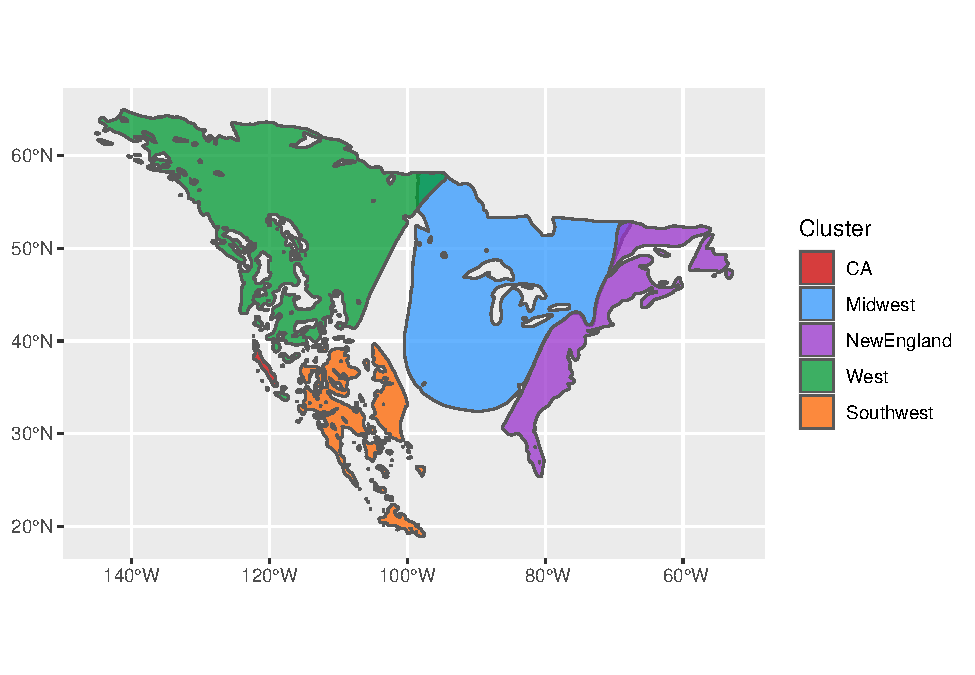
\includegraphics{_main_files/figure-latex/unnamed-chunk-3-1.pdf}

Check which polygons are overlapping. Each row of the output provides a pair of overlapping polygons (if there are any).

\begin{Shaded}
\begin{Highlighting}[]
\FunctionTok{check\_genoscape\_overlap}\NormalTok{(genoscape\_polygon\_sf)}
\end{Highlighting}
\end{Shaded}

\begin{verbatim}
##      [,1]      [,2]        
## [1,] "CA"      "West"      
## [2,] "Midwest" "NewEngland"
## [3,] "Midwest" "West"
\end{verbatim}

\hypertarget{wintering}{%
\chapter{Wintering nodes}\label{wintering}}

For the migratory networks, we will use ecoregions to define the nonbreeding nodes. However, other nonbreeding nodes could be defined by the user instead. If you already have polygons defining your nonbreeding of nodes interest, then move along to \ldots{}

\hypertarget{subsetting-winter-ecoregions}{%
\section{Subsetting winter ecoregions}\label{subsetting-winter-ecoregions}}

The ecoregion data is provided by {[}provide link{]}. The ecoregions are provided in this this package as \texttt{ecoregions\_simple}. We will intersect the ecoregions with the wintering range of the Common Yellowthroat to identify all the ecoregions that overlap with the wintering range.

\begin{Shaded}
\begin{Highlighting}[]
\NormalTok{comyel\_winter }\OtherTok{\textless{}{-}}\NormalTok{ comyel\_range\_smooth }\SpecialCharTok{\%\textgreater{}\%}
\NormalTok{  dplyr}\SpecialCharTok{::}\FunctionTok{filter}\NormalTok{(season }\SpecialCharTok{==} \StringTok{"nonbreeding"}\NormalTok{) }\SpecialCharTok{\%\textgreater{}\%}
\NormalTok{  sf}\SpecialCharTok{::}\FunctionTok{st\_transform}\NormalTok{(}\AttributeTok{crs =} \DecValTok{4326}\NormalTok{) }\SpecialCharTok{\%\textgreater{}\%}
\NormalTok{  sf}\SpecialCharTok{::}\FunctionTok{st\_intersection}\NormalTok{(MuSpTest}\SpecialCharTok{::}\NormalTok{ecoregions\_simple) }\SpecialCharTok{\%\textgreater{}\%}
\NormalTok{  dplyr}\SpecialCharTok{::}\FunctionTok{select}\NormalTok{(Region)}
\end{Highlighting}
\end{Shaded}

\hypertarget{snap-points}{%
\section{Snap points}\label{snap-points}}

Sometimes individuals are not quite within the wintering nodes. Here, we will make sure all sampled individuals get assigned to the nearest ecoregion.

\begin{Shaded}
\begin{Highlighting}[]
\NormalTok{winter.coords }\OtherTok{\textless{}{-}}\NormalTok{ MuSpTest}\SpecialCharTok{::}\NormalTok{coye.winter.meta }\SpecialCharTok{\%\textgreater{}\%}
  \FunctionTok{st\_as\_sf}\NormalTok{(}\AttributeTok{coords=}\FunctionTok{c}\NormalTok{(}\StringTok{"Long"}\NormalTok{,}\StringTok{"Lat"}\NormalTok{)) }\SpecialCharTok{\%\textgreater{}\%}
  \FunctionTok{st\_cast}\NormalTok{(}\StringTok{"MULTIPOINT"}\NormalTok{) }\SpecialCharTok{\%\textgreater{}\%}
  \FunctionTok{st\_set\_crs}\NormalTok{(}\DecValTok{4326}\NormalTok{)}
  
\NormalTok{new.winter.coords }\OtherTok{\textless{}{-}} \FunctionTok{snap\_points}\NormalTok{(winter.coords, comyel\_winter, }\DecValTok{150000}\NormalTok{)}
\end{Highlighting}
\end{Shaded}

\hypertarget{finalize-wintering-nodes}{%
\section{Finalize wintering nodes}\label{finalize-wintering-nodes}}

Now that points have been \emph{snapped} to the appropriate ecoregions, we can further subset all of the ecoregions in which we have actually sampled individuals from. If we haven't sampled individuals from a region, we can't use that region as a node in the migratory connectivity network!

\begin{Shaded}
\begin{Highlighting}[]
\NormalTok{winter\_intersect }\OtherTok{\textless{}{-}} \FunctionTok{st\_intersects}\NormalTok{(comyel\_winter, new.winter.coords, }\AttributeTok{sparse =}\NormalTok{ T)}
\NormalTok{poly\_id }\OtherTok{\textless{}{-}} \FunctionTok{which}\NormalTok{(}\FunctionTok{unlist}\NormalTok{(}\FunctionTok{lapply}\NormalTok{(winter\_intersect, }\ControlFlowTok{function}\NormalTok{(x) }\FunctionTok{length}\NormalTok{(x) }\SpecialCharTok{\textgreater{}} \DecValTok{0}\NormalTok{)))}
\NormalTok{comyel\_winter\_ecoregions }\OtherTok{\textless{}{-}}\NormalTok{ comyel\_winter[poly\_id,]}
\end{Highlighting}
\end{Shaded}

\hypertarget{connectivity}{%
\chapter{Migratory Network Model}\label{connectivity}}

\hypertarget{specifying-relative-abundance}{%
\section{Specifying relative abundance}\label{specifying-relative-abundance}}

To create the network model, we will first specify the relative abundance for each of the nodes (breeding and wintering). This is used to determine the overall importance of the node to the network model. In this example, we will use summarize relative abundance from the seasonal \texttt{ebirdst} rasters we created, but other data could be used as well (for example, habitat suitability from ecological niche models).

For the breeding nodes, we will input the breeding range abundance raster, genoscape polygons, and genoscape cluster names into the \texttt{MuSpTest} function \texttt{get\_abundance\_stats()}. The output will be a data frame of the summarized node suitability.

\begin{Shaded}
\begin{Highlighting}[]
\NormalTok{abd\_season }\OtherTok{\textless{}{-}}\NormalTok{ terra}\SpecialCharTok{::}\FunctionTok{rast}\NormalTok{(}\StringTok{"./comyel/comyel.abd\_season.tif"}\NormalTok{)}

\DocumentationTok{\#\# Breeding}
\NormalTok{cluster\_names }\OtherTok{\textless{}{-}}\NormalTok{ genoscape\_polygon\_sf}\SpecialCharTok{$}\NormalTok{Cluster}
\NormalTok{genoscape\_polygon\_sf }\OtherTok{\textless{}{-}}\NormalTok{ sf}\SpecialCharTok{::}\FunctionTok{st\_read}\NormalTok{(}\StringTok{"./comyel/genoscape/polygons/comyel\_genoscape\_polygon\_sf.shp"}\NormalTok{)}
\NormalTok{breeding\_abundance\_sum }\OtherTok{\textless{}{-}} \FunctionTok{get\_abundance\_stats}\NormalTok{(}\AttributeTok{range\_raster =}\NormalTok{ abd\_season[[}\StringTok{"breeding"}\NormalTok{]],}
                                              \AttributeTok{node\_poly =}\NormalTok{ genoscape\_polygon\_sf,}
                                              \AttributeTok{group\_names =}\NormalTok{ cluster\_names)}
\end{Highlighting}
\end{Shaded}

Similarly for the wintering nodes, we will input the nonbreeding range abundance raster, winter ecoregions, and ecoregion names into the \texttt{MuSpTest} function \texttt{get\_abundance\_stats()}.

\begin{Shaded}
\begin{Highlighting}[]
\DocumentationTok{\#\# Nonbreeding}
\NormalTok{comyel\_winter\_ecoregions }\OtherTok{\textless{}{-}}\NormalTok{ sf}\SpecialCharTok{::}\FunctionTok{st\_read}\NormalTok{(}\StringTok{"./comyel/winter\_regions/comyel\_winter\_ecoregions.shp"}\NormalTok{)}
\NormalTok{ecoregion\_names }\OtherTok{\textless{}{-}}\NormalTok{ comyel\_winter\_ecoregions}\SpecialCharTok{$}\NormalTok{Region}
\NormalTok{nonbreeding\_abundance\_sum }\OtherTok{\textless{}{-}} \FunctionTok{get\_abundance\_stats}\NormalTok{(}\AttributeTok{range\_raster =}\NormalTok{ abd\_season[[}\StringTok{"nonbreeding"}\NormalTok{]],}
                                                 \AttributeTok{node\_poly =}\NormalTok{ comyel\_winter\_ecoregions,}
                                                 \AttributeTok{group\_names =}\NormalTok{ ecoregion\_names)}
\end{Highlighting}
\end{Shaded}

\hypertarget{run-network-model}{%
\section{Run network model}\label{run-network-model}}

\hypertarget{network-visualization}{%
\chapter{Network visualization}\label{network-visualization}}

To be created\ldots{}

  \bibliography{book.bib,packages.bib}

\end{document}
